\documentclass[11pt,a4paper]{article}
\usepackage[T1]{fontenc}
\usepackage[utf8]{inputenc}
\usepackage[polish]{babel}
\usepackage{amsmath}
\usepackage{amsfonts}
\usepackage{graphicx}
\author{Kamil Kuczaj}
\title{Sprawozdanie z Laboratorium 3 - Pomiar czasu znajdywania losowego słowa z listy.\\Implementacja listy, stosu oraz kolejki przy wykorzystaniu odpowiednich interfejsów.}
\date{\today}
\begin{document}

\maketitle

\section{Wstęp}
Podanym zadaniem był pomiar czasu znajdywania losowego elementu listy typu\textit{string}. Należało wykonać pomiary zapisu: $10^1$, $10^3$ oraz $10^5$. Wykorzystano słownik $109582$ najpopularniejszych słów w języku angielskim. Zdecydowano się na wybór języka angielskiego nad polskim z uwagi na zlikwidowanie problemów z wczytywaniem znaków łacińskich. W programie zaimplementowano szablony, dzięki czemu bardzo łatwo jest zmierzyć czas dla innych zmiennych lub nawet własnych klas. 

\section{Specyfikacja komputera}

\begin{center}
	\begin{tabular}{| r | c |}
	\hline
	Wersja kompilatora \textit{g++} & 4.8.4 \\ \hline
	System & Ubuntu 14.04.4 \\ \hline
	Procesor	 & Intel Core i5 2510M 2.3 GHz \\ \hline
	Pamięć RAM & 8 GB DDR3 1600 MHz \\ \hline
	Rozmiar zmiennej \textit{int} & 4 bajty \\ \hline
	\end{tabular}
\end{center}

\newpage

\section{Pomiary}
\bigskip
\begin{figure}[h]
	\centering
		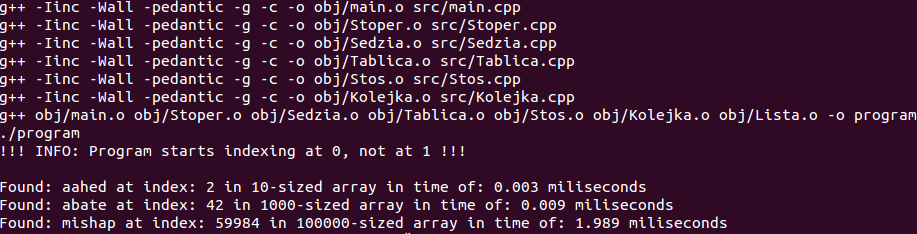
\includegraphics[scale=0.47]{../wykresy/Lista_znajdywanie.png}
		\caption	{Pomiar czasu znajdywania losowego slowa.}	
\end{figure}

\bigskip
\bigskip
\begin{figure}[h]
	\centering
		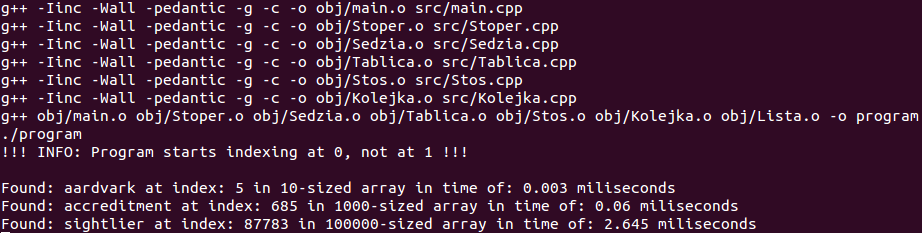
\includegraphics[scale=0.47]{../wykresy/Lista_znajdywanie2.png}
		\caption	{Pomiar czasu znajdywania innego losowego slowa.}	
\end{figure}
\bigskip

Bardzo dużą część czasu zajmowało zapisanie stu tysięcy słów - wynikało to z tego, że należało je zaalokować, a potem wylosować z tej puli. Przeszukiwanie listy było natomiast bardzo krótkie i zwykle nie przekraczało 3 milisekund.

\section{Wnioski}
Zastosowanie struktury danych typu lista zdecydowanie pozwoliło zmniejszyć czas na znalezienie słowa. Zdecydowanie pomogło mi również w tym jak ważne jest zastosowanie odpowiedniej struktury danych do programu.
\end{document}